\documentclass[border=10pt]{standalone}
\usepackage{tikz}
\usepackage{amsmath}
\usepackage{bm} % 加粗红叉需要用到
\usetikzlibrary{arrows.meta}

% 保持你第一段代码的高级配色
\definecolor{inFill}{RGB}{183,224,177}
\definecolor{inLine}{RGB}{32,102,32}
\definecolor{hidFill}{RGB}{199,203,243}
\definecolor{hidLine}{RGB}{52,58,143}
\definecolor{outFill}{RGB}{243,199,199}
\definecolor{outLine}{RGB}{143,52,52}
\definecolor{lineC}{RGB}{38,44,110}
% 新增：过拟合通路的颜色
\definecolor{overfitC}{RGB}{220, 50, 50}

\begin{document}
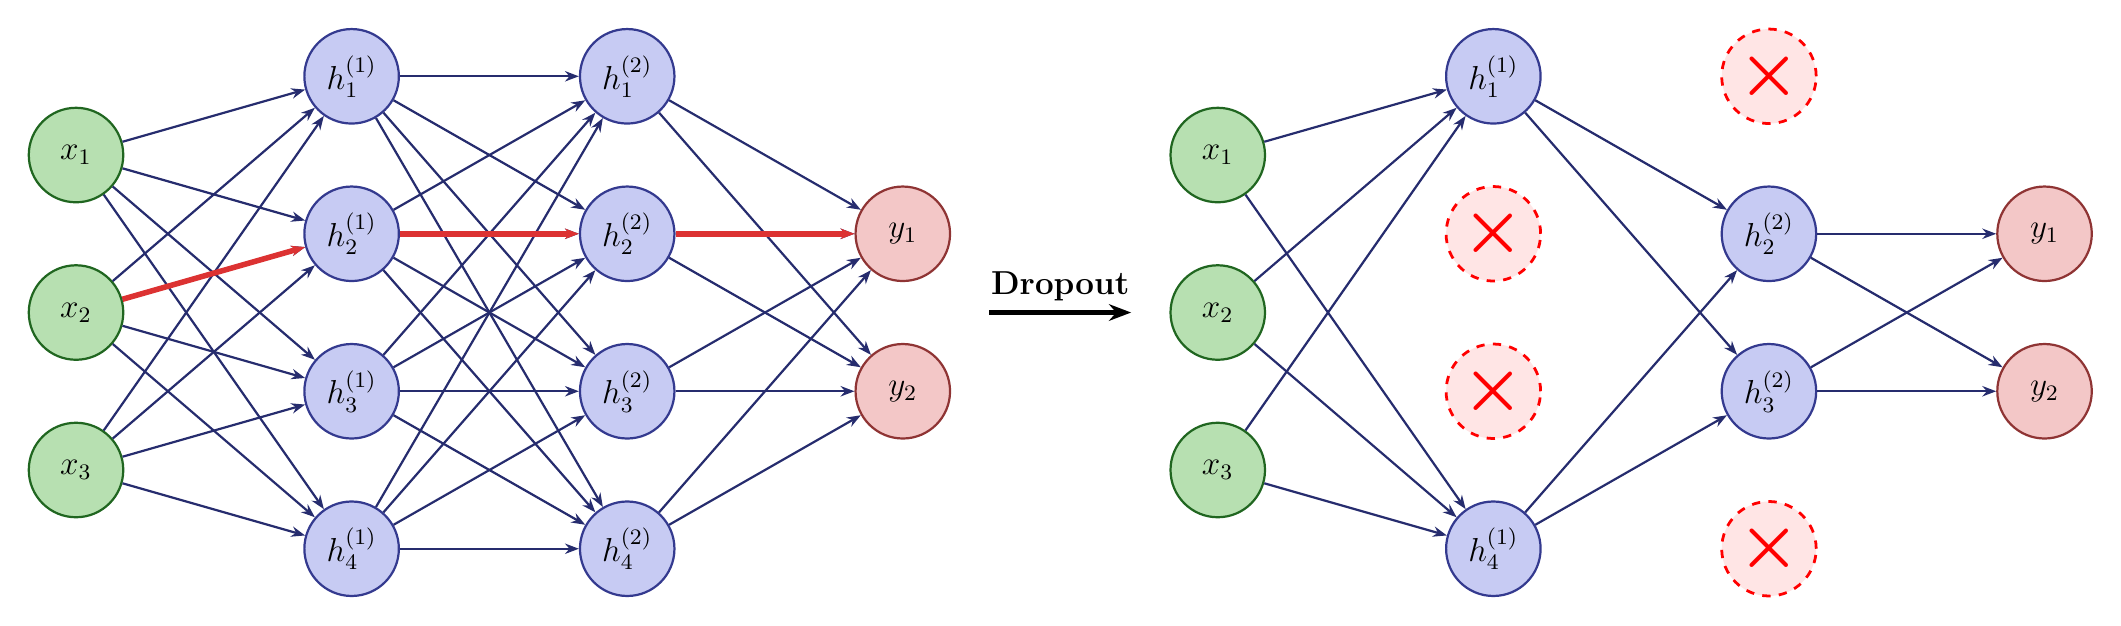
\begin{tikzpicture}[
    >={Stealth[length=5pt]}, line width=0.8pt, font=\large,
    % 统一定义节点样式，统一大小为 1.2cm
    inp/.style={circle, draw=inLine, fill=inFill, minimum size=1.2cm, inner sep=0pt},
    hid/.style={circle, draw=hidLine, fill=hidFill, minimum size=1.2cm, inner sep=0pt},
    outp/.style={circle, draw=outLine, fill=outFill, minimum size=1.2cm, inner sep=0pt},
    % 参考你的要求：被 dropout 杀死的神经元样式（红框，浅红底）
    drop/.style={circle, draw=red, fill=red!10, minimum size=1.2cm, inner sep=0pt, dashed, line width=1pt},
    % 线条样式
    arr/.style={lineC, ->},
    % 过拟合通路线条样式（加粗、醒目颜色）
    overfit/.style={overfitC, ->, line width=2pt}
  ]

  % ==========================================
  % 左侧：标准全连接神经网络 (存在过拟合通路)
  % ==========================================

  % 1. 输入层 (3个节点)
  \node[inp] (x1) at (0, 2)  {$x_1$};
  \node[inp] (x2) at (0, 0)  {$x_2$};
  \node[inp] (x3) at (0,-2)  {$x_3$};

  % 2. 隐藏层 1 (4个节点)
  \node[hid] (h11) at (3.5, 3)  {$h^{(1)}_1$};
  \node[hid] (h12) at (3.5, 1)  {$h^{(1)}_2$};
  \node[hid] (h13) at (3.5,-1)  {$h^{(1)}_3$};
  \node[hid] (h14) at (3.5,-3)  {$h^{(1)}_4$};

  % 3. 隐藏层 2 (4个节点)
  \node[hid] (h21) at (7, 3)  {$h^{(2)}_1$};
  \node[hid] (h22) at (7, 1)  {$h^{(2)}_2$};
  \node[hid] (h23) at (7,-1)  {$h^{(2)}_3$};
  \node[hid] (h24) at (7,-3)  {$h^{(2)}_4$};

  % 4. 输出层 (2个节点)
  \node[outp] (y1) at (10.5, 1)  {$y_1$};
  \node[outp] (y2) at (10.5,-1)  {$y_2$};

  % --- 绘制左侧常规连线 ---
  \foreach \i in {1,2,3} { \foreach \j in {1,2,3,4} { \draw[arr] (x\i) -- (h1\j); } }
  \foreach \i in {1,2,3,4} { \foreach \j in {1,2,3,4} { \draw[arr] (h1\i) -- (h2\j); } }
  \foreach \i in {1,2,3,4} { \foreach \j in {1,2} { \draw[arr] (h2\i) -- (y\j); } }

  % --- 绘制高亮的过拟合通路 (覆盖在常规线上层) ---
  % 通路：x2 -> h1_2 -> h2_2 -> y1
  \draw[overfit] (x2) -- (h12);
  \draw[overfit] (h12) -- (h22);
  \draw[overfit] (h22) -- (y1);

  % ==========================================
  % 中间：Dropout 转换箭头（★ 缩短：12.5~14.5 -> 11.6~13.4）
  % ==========================================
  \draw[-{Stealth[length=8pt]}, line width=1.5pt] (11.6, 0) -- node[above, font=\large\bfseries] {Dropout} (13.4, 0);

  % ==========================================
  % 右侧：应用 Dropout 后的神经网络（★ 整体左移 2：16.5/20/23.5/27 -> 14.5/18/21.5/25）
  % ==========================================

  % 1. 输入层 (保持不变)
  \node[inp] (rx1) at (14.5, 2)  {$x_1$};
  \node[inp] (rx2) at (14.5, 0)  {$x_2$};
  \node[inp] (rx3) at (14.5,-2)  {$x_3$};

  % 2. 隐藏层 1 (杀死第2和第3个)
  \node[hid]  (rh11) at (18, 3)  {$h^{(1)}_1$};
  \node[drop] (rh12) at (18, 1)  {};
  \node[drop] (rh13) at (18,-1)  {};
  \node[hid]  (rh14) at (18,-3)  {$h^{(1)}_4$};
  % 画红叉
  \node[red] at (rh12) {\Huge $\bm{\times}$};
  \node[red] at (rh13) {\Huge $\bm{\times}$};

  % 3. 隐藏层 2 (杀死第1和第4个)
  \node[drop] (rh21) at (21.5, 3)  {};
  \node[hid]  (rh22) at (21.5, 1)  {$h^{(2)}_2$};
  \node[hid]  (rh23) at (21.5,-1)  {$h^{(2)}_3$};
  \node[drop] (rh24) at (21.5,-3)  {};
  \node[red] at (rh21) {\Huge $\bm{\times}$};
  \node[red] at (rh24) {\Huge $\bm{\times}$};

  % 4. 输出层 (保持不变)
  \node[outp] (ry1) at (25, 1)  {$y_1$};
  \node[outp] (ry2) at (25,-1)  {$y_2$};

  % --- 绘制右侧连线 (只连接存活的神经元！) ---
  \foreach \i in {1,2,3} {
      \draw[arr] (rx\i) -- (rh11);
      \draw[arr] (rx\i) -- (rh14);
  }
  \foreach \i in {1,4} {
      \draw[arr] (rh1\i) -- (rh22);
      \draw[arr] (rh1\i) -- (rh23);
  }
  \foreach \i in {2,3} {
      \foreach \j in {1,2} {
          \draw[arr] (rh2\i) -- (ry\j);
      }
  }

\end{tikzpicture}
\end{document}